
\begin{center}
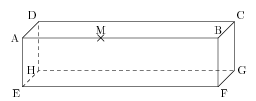
\includegraphics[scale=1]{RepS-39.png} 
\end{center}
\begin{enumerate}
	\item Refais le dessin ci-dessus qui représente un parallélépipède rectangle $ABCDEFGH$.
	\item Sur ce dessin, représente la section de ce pavé par le plan  passant par les points $M$, $C$ et $G$.
	\item Cite toutes les arêtes du pavé parallèles à ce plan.
\end{enumerate}

